\chapter{基于神经网络的着色器程序性能预测方法}

\section{方法总览}

\begin{figure}[h]
  \centering
  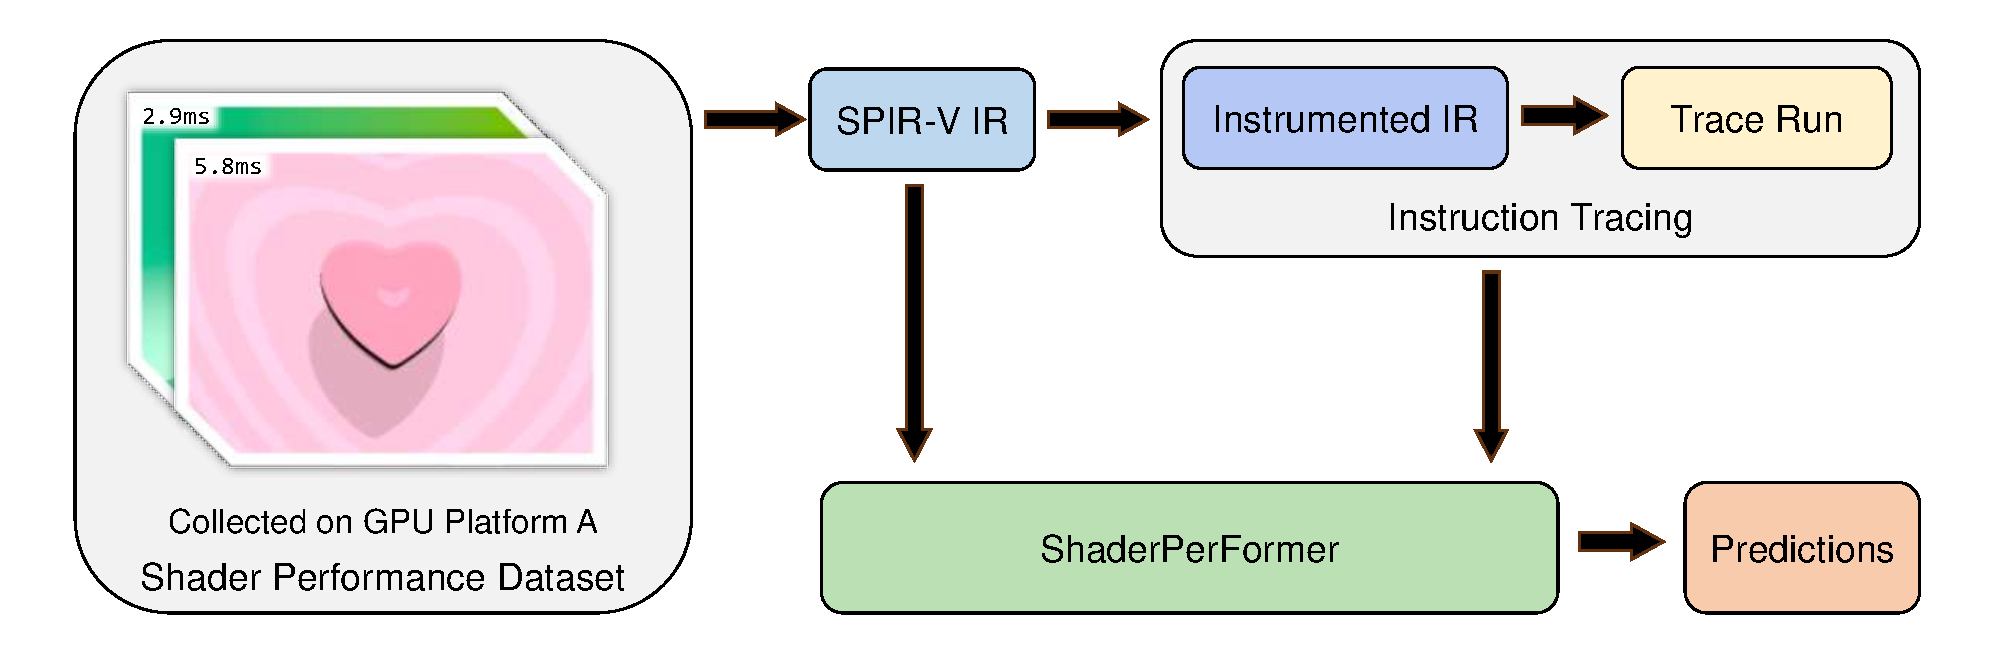
\includegraphics[width=1\linewidth]{figures/OverviewNewNewNew.pdf}
  \caption{本文提出的方法总览。 GPU 平台 A 是待建模的 GPU 平台,本文提出的模型使用 GPU 平台 A 上收集到的性能数据进行训练。}
  % \Description{}
  \label{fig:pipeline_overview}
\end{figure}

% generated by kimi.ai

本研究提出的方法构建了一个针对特定图形处理平台的着色器性能预测模型。该方法可以分为几个主要步骤:着色器数据集构造,着色器指令追踪,以及利用模型进行性能预测。这些环节的大致流程如图 \ref{fig:pipeline_overview} 所示。

首先,为了预测目标图形处理器平台的着色器性能,本方法需要收集一个详尽的着色器性能数据集,该数据集收集过程的具体讨论可以参见第 \ref{sec:dataset} 节。该数据集不仅包含丰富的着色器 GLSL 源代码、编译后的 SPIR-V 中间表示,还包括每次着色器在目标平台运行时着色器的 Uniform 输入参数,以及这些着色器在目标 GPU 平台运行测得的执行时间。这些数据是本方法所述预测器学习理解着色器性能的“原材料”,也为后续的模型训练和验证提供了比较扎实的基础。

数据收集完成后,本文提出的方法的下一个任务是,构建一个基于学习的、能够准确预测着色器在目标 GPU 平台上执行时间的模型。为了达成这个目标,该模型使用两类输入:一是以 SPIR-V 中间表示格式来进行表示的着色器指令;二是与该着色器的指令执行跟踪信息。

原始指令的收集,是通过使用业界标准的着色器编译器 glslang \cite{glslang} 实现的,而着色器执行跟踪信息则是通过一个专门的指令跟踪阶段(见第 \ref{sec:tracing} 节)来获取的。在指令跟踪阶段,本方法提出的过程会对着色器原始的 SPIR-V 中间表示插入额外的跟踪指令,然后运行修改后的中间表示,来统计出执行过程中 SPIR-V 粒度的指令运行计数。这些带有跟踪指令的 SPIR-V 中间表示可以在目标平台运行,也可以在其它非目标平台运行。通过着色器指令跟踪过程,本方法能够较为准确地追踪和分析着色器的执行行为,而无需再在目标平台上实际的执行着色器程序。

随后,本方法将收集到的 SPIR-V 指令和着色器执行跟踪信息一同,输入到构建的神经网络模型 (见第 \ref{sec:model})中。该模型将根据这些输入进行推理,得到对绘制一帧所需的时间的预测。我们利用数据集中的测量的真实值来构造损失函数,从而对模型进行优化。

% generation end

\section{着色器程序性能数据集}

\label{sec:dataset}

% generated by kimi.ai

为了学习着色器程序的性能,我们首先需要丰富的着色器程序。针对这一点,本方法选择利用 Shadertoy \cite{Shadertoy} 平台上用户上传的着色器资源。

Shadertoy 是一个在线平台,它允许用户创建、分享和查看着色器程序及其实现的效果。Shadertoy 平台上的着色器通常假设在顶点阶段处理一个四边形,而所有核心逻辑都在片元阶段执行。这为深入研究片元着色器的性能提供了相对有利的条件。

尽管在渲染时缺乏多样的几何输入,在 Shadertoy 上进行开发的用户仍然可以通过应用如 Ray Marching \cite{Hart1996}, 过程化内容生成 (Procedural Content Generation) 等技术来创建能够产生复杂视觉效果的着色器。图 \ref{fig:shadertoy_gallery} 展示了一些 Shadertoy 中着色器使用的技术和使用的技术路线。

\begin{figure}[htbp]
     \centering
     \begin{subfigure}[b]{300}
         \centering
         
\includegraphics[width=\textwidth]{figures/shadertoy_cloud.png}
         \caption{$y=x$}
         \label{fig:y equals x}
     \end{subfigure}
     \hfill
     \begin{subfigure}[b]{300}
         \centering
         
\includegraphics[width=\textwidth]{figures/shadertoy_cloud.png}
         \caption{$y=3\sin x$}
         \label{fig:three sin x}
     \end{subfigure}
        \caption{Three simple graphs}
        \label{fig:three graphs}
\end{figure}


这些着色器的性能表现在相关文献 \cite{https://doi.org/10.1111/cgf.14457} 中有所探讨。因此,本方法认为Shadertoy上的着色器在片元着色器性能建模方面具有代表性。

\paragraph{收集}
本方法通过Shadertoy网站提供的API接口,收集了27911个着色器。

\paragraph{编译}
从Shadertoy下载的着色器包含一个名为 \verb|mainImage| 的入口函数。本方法将 \verb|mainImage| 封装为片元着色器的入口点,并在统一块中引入如 \verb|iTime| 和 \verb|iResolution| 等 Uniform 变量。随后,使用glslang编译器将这些着色器编译为SPIR-V中间表示。

\paragraph{性能分析}
本方法开发了一个名为 \verb|vkExecute| 的Python扩展来测量着色器的性能。核心的性能分析逻辑在算法~\ref{alg:profile} 中详细描述。为了减少CPU提交的开销,本方法采用基于GPU的时间戳计数器来精确测量执行时间。\verb|unitTs| 表示计数器每次增加所对应的时间间隔,这一值依赖于具体的硬件平台。为了进一步降低GPU绘制的开销,本方法在时间戳计数器读取之间额外发出 \verb|num_cycles| 次绘制命令(见概念\label{concept:numCycles}),因为许多收集到的着色器在现代 GPU 平台上的执行速度非常快(>1000fps)。此外,为了确保结果的准确性,本方法进行了 \verb|num_trials| 次 GPU 命令提交(见概念\label{concept:numTrials}),并将所有测量结果存储以供后续分析。在所有性能分析过程中,本方法通过供应商提供的接口锁定了测试平台上的着色器和内存时钟频率。

\paragraph{错误恢复}
Shadertoy平台并不对用户提交的着色器进行合法性验证,因此编译错误在所难免。同时,由于着色器已经成为图灵完备的领域特定语言(DSL),其执行时间可能没有上限,这可能导致现代 GPU 驱动程序在渲染命令耗时过长时触发引擎或 GPU 的重置。当此类重置事件发生时,分析器的 Vulkan 上下文可能会失效。为了避免管理程序被意外终止,本方法将着色器性能分析任务分散到多个独立进程中进行。

% generate end

\begin{algorithm}
\caption{性能分析例程伪代码}
\label{alg:profile}

\SetAlgoLined % For setting line numbering
\SetKwFunction{FProfileShaderOnce}{ProfileShaderOnce}
\SetKwFunction{FProfileShader}{ProfileShader}
\SetKwProg{Fn}{Function}{:}{}
\SetKwInOut{Input}{input} \SetKwInOut{Output}{output}

\Fn{\FProfileShaderOnce{$num\_cycles$}}{
    Do image memory barrier, layout transition and reset timestamp query pool\;
    Wait for previous commands to finish\;
    $cmdBuf \gets$ allocateCmdBufFromPool()\;
    Emit write timestamp $ts_1$ command into $cmdBuf$\;
    \For{$i \gets 1$ \textbf{to} $num\_cycles$}{
        Emit bind graphics pipeline and descriptors command into $cmdBuf$\;
        Emit draw command into $cmdBuf$\;
    }
    Emit write timestamp $ts_2$ command into $cmdBuf$\;
    Submit to command queue\;
    Wait for previous command to finish\;
    \Return $(ts_2 - ts_1) \times unitTs$\;
}

\Fn{\FProfileShader{$num\_cycles$, $num\_trials$}}{
    $results \gets []$\;
    \For{$i \gets 1$ \textbf{to} $num\_trials$}{
        $results[i] \gets$ \FProfileShaderOnce{$num\_cycles$}\;
    }
    \Return $results$\;
}

\end{algorithm}

% \begin{algorithm}
% \caption{Pseudocode for the profiling routine}
% \label{alg:profile}
% \begin{algorithmic}[1] % The number tells where the line numbering should start
%   \Function{ProfileShaderOnce}{$num\_cycles$} % Algorithm name and parameters
%     \State Do image memory barrier, layout transition and reset timestamp query pool
%     \State Wait for previous commands to finish
%     \State $cmdBuf \gets $ allocateCmdBufFromPool() 
%     \State Emit write timestamp $ts_1$ command into $cmdBuf$
%     \For{$i \gets 1$ \textbf{to} $num\_cycles$}
%       \State Emit bind graphics pipeline and descriptors command into $cmdBuf$
%       \State Emit draw command into $cmdBuf$
%     \EndFor
%     \State Emit write timestamp $ts_2$ command into $cmdBuf$
%     \State Submit to command queue
%     \State Wait for previous command to finish
%     \State \Return $(ts_2 - ts_1) \times unitTs$ 
%   \EndFunction
%   \Function{ProfileShader}{$num\_cycles$, $num\_trials$}
%     \State $results \gets []$
%     \For{$i \gets 1$ \textbf{to} $num\_trials$}
%         \State $results[i] \gets$ ProfileShaderOnce($num\_cycles$)
%     \EndFor
%     \State \Return $results$
%   \EndFunction
% \end{algorithmic}
% \end{algorithm}


% TODO: add code snippet

\section{基本块粒度的 SPIR-V 指令追踪}

\label{sec:tracing}

\subsection{基本块}

\subsection{着色器程序输入}

\subsection{SPIR-V 指令编排}

\section{着色器程序性能模型}

\label{sec:model}

\subsection{SPIR-V 分词器}

\subsection{指令计数上下文嵌入}

\subsection{编解码和输出层}

\section{实验和分析}

\subsection{性能数据集分布分析}

% \subsection{环境设置}

% \subsection{源码分布分析}

% \subsection{时间分布分析}

\subsection{性能模型预测结果分析}

% \subsection{环境设置}

% \subsection{模型预测结果分析}

% \subsection{指令追踪信息对预测的影响}

\subsection{指令追踪信息对预测的影响}
